%% Early Forecasting of Catastrophic Forgetting in CLIP Fine-Tuning
%% ACDSA 2027 two-column manuscript (IEEE conference template).
\documentclass[10pt,conference]{IEEEtran}
\usepackage{paperstyle}

\graphicspath{{figures/}}
\DeclareMathOperator*{\argmin}{arg\,min}

\begin{document}

\title{Early Forecasting of Catastrophic Forgetting in CLIP Fine-Tuning}

\author{
\IEEEauthorblockN{Saanvi Eha Chandra\equalcontrib}
\IEEEauthorblockA{Nexus Labs\\ Palo Alto, USA}
\and
\IEEEauthorblockN{Avni Gautam\equalcontribmark}
\IEEEauthorblockA{Nexus Labs\\ Palo Alto, USA}
\and
\IEEEauthorblockN{Krisha Gupta\equalcontribmark}
\IEEEauthorblockA{Nexus Labs\\ Palo Alto, USA}
\and
\IEEEauthorblockN{Neel Ranadive\equalcontribmark}
\IEEEauthorblockA{Nexus Labs\\ Palo Alto, USA}
\and
\IEEEauthorblockN{Aarav Shah\equalcontribmark}
\IEEEauthorblockA{Nexus Labs\\ Palo Alto, USA}
\and
\IEEEauthorblockN{Noah Yoo\equalcontribmark}
\IEEEauthorblockA{Nexus Labs\\ Palo Alto, USA}
\and
\IEEEauthorblockN{Srikanth Samy}
\IEEEauthorblockA{University of California, Berkeley\\ Berkeley, USA\\ ssamy@berkeley.edu}
\and
\IEEEauthorblockN{Ishaan Gupta}
\IEEEauthorblockA{Stanford University\\ Stanford, USA\\ ishaangupta@stanford.edu}
}

\maketitle

\begin{abstract}
Fine-tuning a vision--language model on a narrow dataset improves the target task while
eroding the zero-shot competence that made the model valuable. We ask whether the
\emph{final} magnitude of that erosion can be forecast from a short warm-up of the
fine-tuning run. Our experiment comprises $48$ fine-tuning runs of CLIP ViT-B/32
($16$ specialised datasets $\times$ $3$ learning rates $\times$ $20$ epochs), logging
five trajectory signals after every epoch and measuring forgetting as the mean drop in
zero-shot accuracy over CIFAR-100, CIFAR-10, and STL-10. Forecasters are evaluated by
leave-one-dataset-out cross-validation, so that all three learning-rate runs of a
held-out dataset are unseen. Four cheap pre-training descriptors alone reach
$R^2=0.43$; adding a five-epoch warm-up raises this to $R^2=0.92$ and cuts mean absolute
error from $0.070$ to $0.025$. Simple tabular regressors beat both an MLP
($R^2=-0.66$) and an LSTM ($R^2=0.81$) in this $48$-row, $16$-group regime. Critically,
we add the persistence control that the underlying study identified as missing:
predicting final forgetting to equal forgetting at the end of the warm-up already
attains $R^2=0.85$ and Spearman $\rho=0.945$. The learned forecaster's advantage over
naive curve continuation is therefore real but narrow, and it is confined to very short
warm-ups ($K\le5$); beyond $K\approx6$ the two are indistinguishable. We conclude that
most of the ``forecasting'' signal is trajectory persistence, and that future work in
this area must report a persistence baseline to make a meaningful claim.
\end{abstract}

\paperkeywords{Catastrophic forgetting, CLIP, fine-tuning dynamics, grouped
cross-validation, multimodal learning, transfer learning, zero-shot classification.}

\section{Introduction}
Contrastively pretrained vision--language models such as
CLIP~\cite{radford2021clip} derive their practical value from breadth: a single set of
weights classifies arbitrary categories by comparing image embeddings against text
prompts, with no task-specific training. Practitioners routinely trade that breadth for
depth by fine-tuning on a specialised corpus. The weights that encode the specialised
task are the same weights that encoded everything else, and updating them overwrites
prior competence---the phenomenon known as catastrophic
forgetting~\cite{mccloskey1989,kirkpatrick2017ewc}.

The economics are unfavourable. A fine-tuning campaign is paid for in advance, but the
damage is measured afterwards. If the eventual loss of general capability could be
estimated from a short prefix of the run, a practitioner could abort, reduce the
learning rate, or switch to a robustness-preserving procedure such as weight-space
interpolation~\cite{wortsman2022wiseft,ilharco2022patching} before most of the compute
is spent.

Prior work predicts forgetting from static properties of the pretrained model and target
dataset. We ask a different question:

\begin{quote}
\emph{Given the first $K$ epochs of a fine-tuning run on a dataset never seen before,
how accurately can the final forgetting be forecast---and how much of that accuracy is
anything more than extrapolating the curve?}
\end{quote}

The second clause is the part most easily neglected. A forecaster that consumes
$\Phi_K$, the forgetting already observed at epoch $K$, as an input feature is in
competition not with an uninformed prior but with the trivial rule $\hat\Phi_T=\Phi_K$.
We report that comparison explicitly, and it substantially tempers the headline.

\subsection{Contributions}
\begin{enumerate}
\item A cached, fully reproducible $48$-run fine-tuning campaign that logs five
      trajectory signals per epoch across $16$ datasets spanning three visual domains
      and three learning rates.
\item A grouped (leave-one-dataset-out) forecasting benchmark in which every
      normalisation and model fit occurs inside the fold, comparing five estimator
      families under a static-only versus static-plus-warm-up ablation.
\item \textbf{A persistence control.} We show that $\hat\Phi_T=\Phi_K$ reaches
      $R^2=0.85$, so that the learned forecaster's $R^2=0.92$ represents a
      $0.07$ improvement over curve continuation rather than the $0.49$ improvement
      suggested by the static-only ablation alone.
\item A characterisation of \emph{where} learning helps: the learned model dominates
      persistence only for $K\le5$, the regime where aborting a run still saves
      meaningful compute.
\end{enumerate}

\section{Experimental Design}

\subsection{Model and forgetting definition}
All runs start from CLIP ViT-B/32 with the original OpenAI pretrained weights
($151.3$M parameters). Zero-shot classification follows the standard prompt-ensembling
recipe: for class names $c_1,\dots,c_M$ we build prompts
$\texttt{"a photo of a }c_m\texttt{."}$, encode them with the text tower, $\ell_2$-
normalise, and predict
\begin{equation}
\hat{y}(\mathbf{x}) \;=\; \argmin_{m}\; -\,
\frac{f_{\mathrm{img}}(\mathbf{x})^{\!\top} g_{\mathrm{txt}}(c_m)}
     {\lVert f_{\mathrm{img}}(\mathbf{x})\rVert\;\lVert g_{\mathrm{txt}}(c_m)\rVert}.
\label{eq:zeroshot}
\end{equation}

Let $\mathcal{B}=\{\text{CIFAR-100},\text{CIFAR-10},\text{STL-10}\}$ be held-out general
benchmarks, and $A_b^{(0)}$ the pretrained zero-shot accuracy on $b\in\mathcal{B}$. We
measure $A_b^{(0)}=0.617$, $0.861$, and $0.956$ respectively. Forgetting after epoch
$t$ is the mean accuracy loss,
\begin{equation}
\Phi_t \;=\; \frac{1}{|\mathcal{B}|}\sum_{b\in\mathcal{B}}\left(A_b^{(0)}-A_b^{(t)}\right).
\label{eq:forgetting}
\end{equation}
$\Phi_t>0$ denotes lost general capability; $\Phi_t<0$ would denote improvement. The
prediction target is $\Phi_T$ with $T=20$.

\subsection{Fine-tuning protocol}
For each dataset $d$ and learning rate $\eta$ we reset the encoder to pretrained
weights, attach a freshly initialised linear head $W_d\in\mathbb{R}^{K_d\times512}$, and
minimise cross-entropy over both the image tower and the head with
AdamW~\cite{loshchilov2019adamw}:
\begin{equation}
\mathcal{L}_{\mathrm{ft}}
 = -\frac{1}{N}\sum_{i=1}^{N}\log
   \frac{\exp\!\big(W_{d,y_i}^{\!\top} f_{\mathrm{img}}(\mathbf{x}_i)\big)}
        {\sum_{k}\exp\!\big(W_{d,k}^{\!\top} f_{\mathrm{img}}(\mathbf{x}_i)\big)} .
\label{eq:finetune}
\end{equation}
The encoder uses learning rate $\eta\in\{10^{-6},5\times10^{-6},10^{-5}\}$, the head
uses $10^{-3}$, weight decay is $10^{-4}$, batch size is $128$, and every dataset is
subsampled to an identical budget of $4000$ training images so that a large corpus
cannot appear to cause more forgetting merely by supplying more gradient steps. This
yields $16\times3=48$ runs of $20$ epochs.

\subsection{Datasets}
The $16$ target datasets fall into three families by visual distance from web
photography: \emph{natural} (OxfordPets, Food101, FGVCAircraft, DTD, EuroSAT),
\emph{digits} (SVHN, MNIST, GTSRB), and \emph{medical} (eight MedMNIST
collections~\cite{yang2023medmnist}). The medical and digit sets are natively $28\times28$
or $32\times32$ and must be upsampled roughly eightfold to CLIP's $224\times224$ input,
which introduces a systematic blur absent from the natural family.

\subsection{Logged signals}
After every epoch we record five quantities. Beyond $\Phi_t$ and the training loss and
accuracy, two measure how far the network has physically moved from its initialisation:
\begin{align}
\delta^{\mathrm{par}}_t &= \frac{\lVert \boldsymbol{\theta}_t-\boldsymbol{\theta}_0\rVert_2}
                                {\lVert \boldsymbol{\theta}_0\rVert_2}, \label{eq:pdrift}\\[2pt]
\delta^{\mathrm{emb}}_t &= \mathbb{E}_{\mathbf{x}\sim\mathcal{P}}
   \left[\,1-\cos\!\big(f_t(\mathbf{x}),\,f_0(\mathbf{x})\big)\right], \label{eq:edrift}
\end{align}
where $\mathcal{P}$ is a fixed probe set of general images. Equation~\eqref{eq:pdrift}
is parameter drift, \eqref{eq:edrift} is representation drift. Both are plausible early
proxies for damage, because forgetting is ultimately a consequence of the encoder's
outputs moving away from the geometry the text tower was aligned to.

\section{Observed Forgetting}

\subsection{Trajectories}
\cref{fig:curves} shows all $48$ forgetting trajectories. Two effects are immediate and
large. First, forgetting scales sharply with the learning rate: at $\eta=10^{-6}$ almost
every dataset ends below $\Phi_{20}=0.10$, whereas at $\eta=10^{-5}$ several exceed
$0.35$, i.e.\ more than a third of the pretrained general accuracy is destroyed.
Second, curves are monotone and saturating for essentially every run, which is precisely
the property that later makes naive persistence a strong forecaster.

\begin{figure*}[!t]
\centering
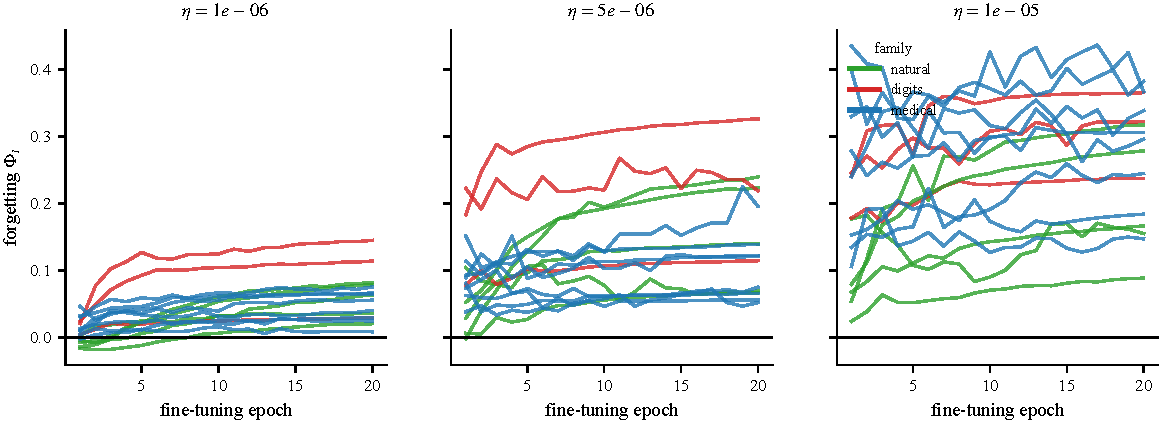
\includegraphics[width=\textwidth]{fig1_forgetting_curves.pdf}
\caption{Forgetting $\Phi_t$ during fine-tuning for all $16$ datasets at the three
learning rates. Colour encodes dataset family. Curves are near-monotone and saturating,
which is the structural reason a persistence forecaster performs well.}
\label{fig:curves}
\end{figure*}

\subsection{Which datasets forget most}
\cref{fig:final} ranks final forgetting at the largest learning rate and summarises it
by family. Family means are $0.309$ (digits), $0.283$ (medical), and $0.201$ (natural),
with ranges given in \cref{tab:family}. The ordering partially matches the naive
expectation that visually distant data causes more damage, but the medical family spans
almost the entire observed range ($0.147$ to $0.382$), so ``distance from web photos''
is not by itself a sufficient predictor.

\begin{table*}[!t]
\centering
\caption{Final forgetting $\Phi_{20}$ at $\eta=10^{-5}$, grouped by dataset family.}
\label{tab:family}
\begin{tabular}{lrrrr}
\toprule
Family & Datasets & Mean & Min & Max\\
\midrule
digits  & 3 & 0.309 & 0.238 & 0.366\\
medical & 8 & 0.283 & 0.147 & 0.382\\
natural & 5 & 0.201 & 0.089 & 0.318\\
\bottomrule
\end{tabular}
\end{table*}

\begin{figure*}[!t]
\centering
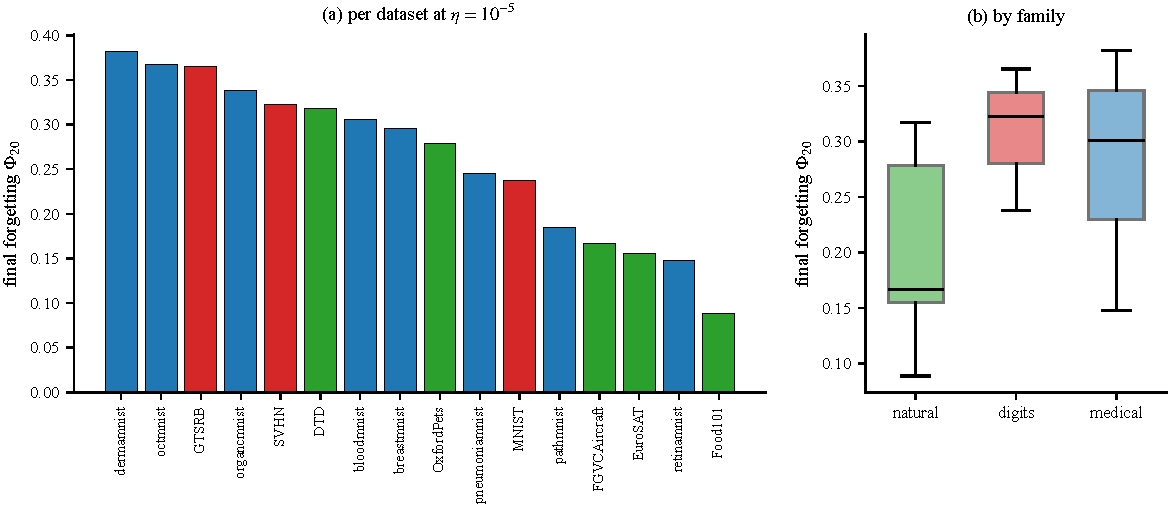
\includegraphics[width=\textwidth]{fig2_final_forgetting.pdf}
\caption{(a) Final forgetting per dataset at $\eta=10^{-5}$, coloured by family.
(b) Distribution by family. The medical family is highly dispersed, so family membership
alone is a weak predictor.}
\label{fig:final}
\end{figure*}

\section{Forecasting Setup}

\subsection{Features}
Each of the $48$ runs becomes one row. The \emph{static} block $\mathbf{s}_d$ contains
four descriptors computed before any training, plus $\log_{10}\eta$:
\begin{itemize}
\item \texttt{semantic\_dist}: $1-$ pretrained zero-shot accuracy on $d$;
\item \texttt{clip\_embed\_dist}: distance between the mean CLIP embedding of $d$ and
      that of general photography;
\item \texttt{spectral\_dist}: a model-free Fourier-domain texture discrepancy;
\item \texttt{frechet\_dist}: a Fr\'echet distribution distance in embedding
      space~\cite{heusel2017fid}.
\end{itemize}
The \emph{warm-up} block $\mathbf{w}_d^{(K)}$ summarises the first $K$ epochs by the
terminal value of each logged signal together with the fitted slope of the forgetting
curve,
\begin{equation}
\hat{\beta}_K=\frac{\sum_{t=1}^{K}(t-\bar{t})\left(\Phi_t-\bar{\Phi}\right)}
                   {\sum_{t=1}^{K}(t-\bar{t})^{2}} .
\label{eq:slope}
\end{equation}
\cref{fig:features} (a) shows that individual static descriptors correlate only weakly
with the outcome ($|r|\le0.44$, $n=16$), motivating multivariate models; panel (b)
shows the co-evolution of the logged signals within a single run.

\begin{figure*}[!t]
\centering
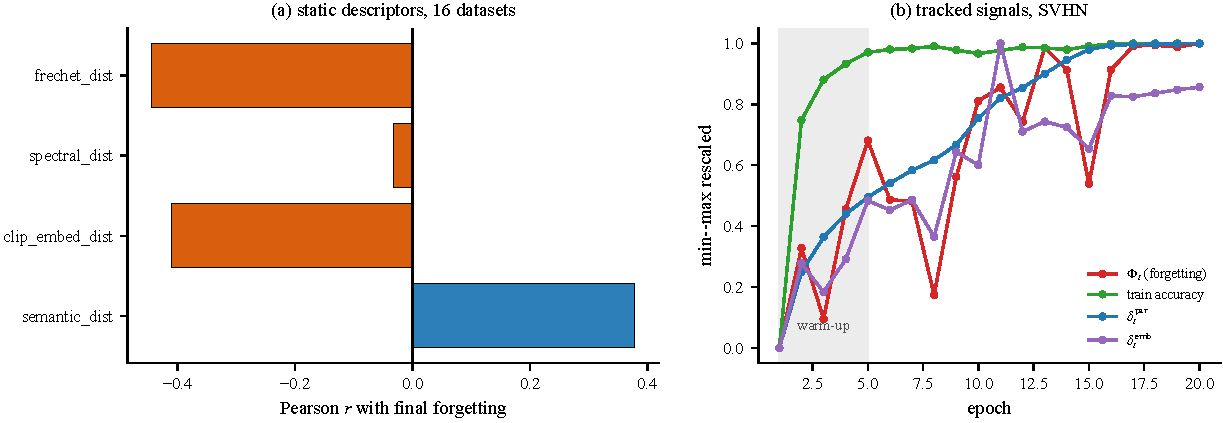
\includegraphics[width=\textwidth]{fig3_features.pdf}
\caption{(a) Pearson correlation of each static descriptor with final forgetting across
the $16$ datasets. All are modest and estimated from $16$ points. (b) The four tracked
signals for SVHN at $\eta=10^{-5}$, min--max rescaled; the shaded region is the
$K=5$ warm-up.}
\label{fig:features}
\end{figure*}

\subsection{Grouped evaluation}
The three learning-rate runs of one dataset share $\mathbf{s}_d$ exactly and are
statistically dependent. Random row splitting would therefore leak dataset identity and
inflate scores~\cite{cawley2010overfitting}. We use leave-one-dataset-out: for each
$d^\star$ the forecaster is fitted on the $45$ rows from the other $15$ datasets and
predicts the $3$ held-out rows. Feature standardisation---and, for the LSTM, sequence
normalisation---is fitted on the training datasets only.

\subsection{Estimators and controls}
Four tabular regressors are compared: ridge regression with generalised
cross-validated penalty~\cite{hoerl1970ridge}, a $300$-tree random
forest~\cite{breiman2001rf}, gradient boosting with depth-2
stumps~\cite{friedman2001gbm}, and a $(32,16)$ MLP. A single-layer
LSTM~\cite{hochreiter1997lstm} over the raw warm-up sequence, concatenated with the
static block, is evaluated separately because it consumes the warm-up in ordered form.
All are implemented in scikit-learn~\cite{pedregosa2011sklearn} except the LSTM.

We additionally define two \emph{model-free} controls, which are the methodological
core of this paper:
\begin{align}
\text{Persistence:}\quad & \hat\Phi_T=\Phi_K, \label{eq:persist}\\
\text{Slope extrapolation:}\quad & \hat\Phi_T=\Phi_K+\hat{\beta}_K\,(T-K). \label{eq:extrap}
\end{align}
Neither is fitted to anything. Any learned forecaster that consumes $\Phi_K$ must beat
\eqref{eq:persist} to have demonstrated that it learned something beyond the fact that
forgetting curves keep going.

Scores are mean absolute error, Spearman rank correlation, and
$R^2=1-\sum(\hat\Phi-\Phi)^2/\sum(\Phi-\bar\Phi)^2$, all computed over the pooled
out-of-fold predictions.

\section{Results}

\subsection{The warm-up ablation}
\cref{tab:main} and \cref{fig:quality}(a) give the central comparison. With static
features alone, ridge regression reaches $R^2=0.426$ and the tree ensembles $0.29$--$0.39$;
this is genuine but weak signal, consistent with the modest univariate correlations of
\cref{fig:features}(a). Adding the five-epoch warm-up moves all three well-behaved
models to $R^2\approx0.91$--$0.92$ and reduces MAE from roughly $0.070$ to $0.025$,
a $2.8\times$ error reduction. \cref{fig:quality}(b) shows the predicted-versus-actual
scatter for the best model: held-out datasets from all three families lie close to the
identity line, with no systematic family bias.

\begin{table*}[!t]
\centering
\caption{Leave-one-dataset-out forecasting of final forgetting $\Phi_{20}$, $K=5$.
Rows above the rule are fitted models; rows below are model-free controls that consume
no training data at all. Best fitted $R^2$ in bold.}
\label{tab:main}
\begin{tabular}{llrrr}
\toprule
Inputs & Estimator & MAE & Spearman $\rho$ & $R^2$\\
\midrule
\multirow{4}{*}{static only}
 & Ridge          & 0.070 & 0.683 & 0.426\\
 & Random forest  & 0.070 & 0.670 & 0.394\\
 & Grad.\ boosting& 0.075 & 0.614 & 0.294\\
 & MLP            & 0.122 & 0.346 & $-1.133$\\
\addlinespace
\multirow{5}{*}{static $+$ warm-up}
 & Ridge          & 0.025 & 0.920 & 0.911\\
 & Random forest  & 0.025 & 0.928 & 0.912\\
 & Grad.\ boosting& 0.025 & 0.924 & \textbf{0.917}\\
 & LSTM           & 0.038 & 0.878 & 0.812\\
 & MLP            & 0.113 & 0.481 & $-0.660$\\
\midrule
\multirow{2}{*}{control}
 & Persistence, Eq.~\eqref{eq:persist}        & 0.034 & 0.945 & 0.848\\
 & Slope extrap., Eq.~\eqref{eq:extrap}       & 0.133 & 0.634 & $-2.281$\\
\bottomrule
\end{tabular}
\end{table*}

\begin{figure*}[!t]
\centering
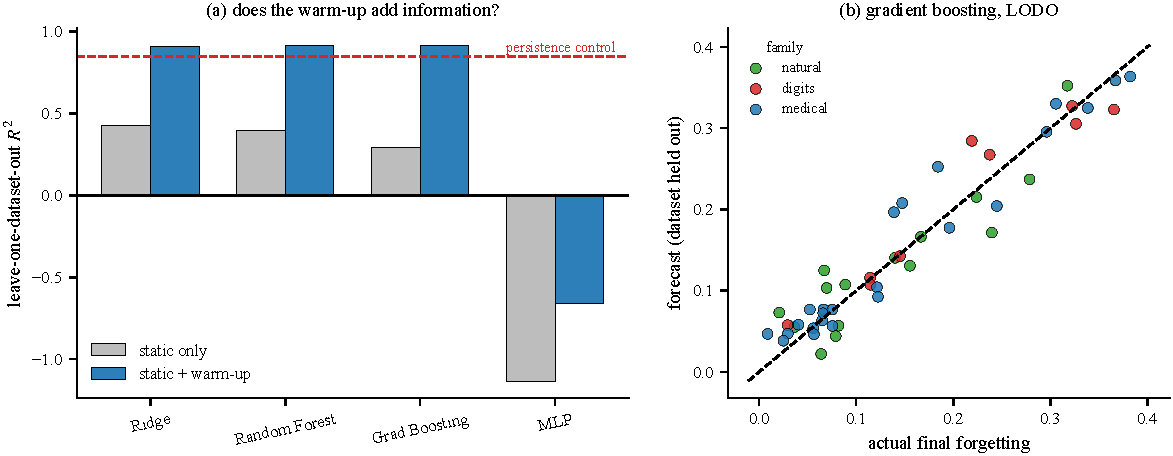
\includegraphics[width=\textwidth]{fig4_forecast_quality.pdf}
\caption{(a) Leave-one-dataset-out $R^2$ with and without the warm-up block; the dashed
red line is the persistence control of Eq.~\eqref{eq:persist}, which no static-only model
approaches and which the warm-up models beat by only $\approx0.07$.
(b) Predicted versus actual final forgetting for gradient boosting; each point is one
held-out run.}
\label{fig:quality}
\end{figure*}

\subsection{The persistence control changes the interpretation}
Read without a control, \cref{tab:main} tells a strong story: watching five of twenty
epochs more than doubles $R^2$. The persistence control reframes it. The rule
``final forgetting equals forgetting at epoch $5$'' attains $R^2=0.848$, MAE $0.034$,
and---strikingly---the \emph{highest} rank correlation in the entire table,
$\rho=0.945$. The best learned forecaster improves $R^2$ by $0.069$ and MAE by $0.009$,
and is actually \emph{worse} at ranking which dataset will forget most.

This is not a negative result about the study; it is a precise localisation of what the
learned model contributes. Persistence systematically underestimates, because $\Phi_t$
is still rising at $t=5$. The learned models supply the missing magnitude correction,
which is exactly the kind of calibration a regression can learn from $45$ neighbouring
runs. What they do not supply is new information about the \emph{ordering} of datasets,
which the warm-up already encodes.

Slope extrapolation, Eq.~\eqref{eq:extrap}, fails badly ($R^2=-2.281$). Because the
forgetting curves are concave, linearly continuing the early slope massively
overestimates the endpoint. The failure is instructive: it shows that the warm-up's
predictive content is in its \emph{level}, not in its derivative, and that a plausible
hand-crafted rule can be far worse than either the naive rule or the learned one.

\subsection{How early is early enough?}
\cref{fig:warmup} sweeps the warm-up length $K$ and re-runs the entire evaluation at
each value, including both controls. Three regimes are visible.

\begin{figure*}[!t]
\centering
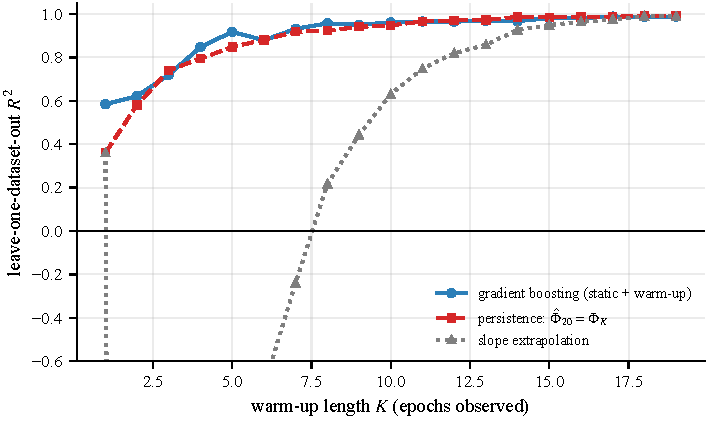
\includegraphics[width=0.72\textwidth]{fig5_warmup_length.pdf}
\caption{Forecast quality against warm-up length $K$. The learned forecaster's advantage
over persistence is confined to $K\le5$; from $K\approx6$ onward the two curves are
interchangeable. Slope extrapolation is catastrophic for small $K$ and only becomes
competitive once there is almost nothing left to forecast.}
\label{fig:warmup}
\end{figure*}

For $K\le5$ the learned model leads clearly: at $K=4$ it attains $R^2=0.848$ against
persistence's $0.795$, and at $K=5$, $0.917$ against $0.848$. This is the operationally
useful window, in which $75$--$80\%$ of the run remains and aborting saves real compute.
For $6\le K\le10$ the two curves interleave within $\pm0.03$ and neither dominates. For
$K\ge11$ both exceed $R^2=0.96$ and the forecasting problem has essentially dissolved:
by then the curve has nearly saturated, so predicting the endpoint is close to reading it.

The practical recommendation follows directly. If the goal is an early-abort signal, use
$K\approx5$ and use a fitted model, because that is where fitting pays. If $K$ can be
larger, do not bother fitting anything.

\subsection{Small samples punish flexible models}
The MLP is worse than predicting the mean in both feature settings
($R^2=-1.13$ and $-0.66$), and the LSTM, despite consuming strictly more information
than the tabular models (the ordered sequence rather than its endpoint), scores $0.812$
against gradient boosting's $0.917$. With $45$ training rows drawn from $15$ independent
groups, the effective sample size is far below what either architecture needs. This is a
clean instance of a general rule: capacity is only an asset when the group count, not the
row count, supports it.

\section{Discussion}

\subsection{What is supported}
\begin{enumerate}
\item Final forgetting varies by more than a factor of four across datasets and learning
      rates in this campaign ($\Phi_{20}$ from $0.089$ to $0.382$ at $\eta=10^{-5}$).
\item Early training dynamics carry substantially more forecast signal than the four
      static descriptors: $R^2$ rises from $0.43$ to $0.92$ under leave-one-dataset-out
      evaluation.
\item \emph{Most of that signal is persistence.} A zero-parameter rule reaches
      $R^2=0.85$ and the best rank correlation observed. The learned contribution is a
      magnitude correction worth $\approx0.07$ $R^2$, concentrated at $K\le5$.
\item Simple regularised estimators dominate an MLP and an LSTM at this sample size.
\end{enumerate}

\subsection{Threats to validity}
The independent unit is a dataset, so the effective sample size for a generalisation
claim is $16$, not $48$; second and third decimal places in \cref{tab:main} are not
stable evidence. The campaign uses one architecture, one optimiser, one prompt template,
and one run per configuration, with no seed replication, so run-to-run variance is
unmeasured and is confounded with between-dataset variance. The three general benchmarks
in $\mathcal{B}$ are all small natural-image classification sets, so $\Phi$ measures loss
of one particular kind of general competence rather than of general competence as such.
Finally, the static descriptors and the warm-up features were designed together with the
campaign, so their relative merit is not an unbiased comparison against the literature's
static predictors.

\subsection{Recommendations for future work}
The decisive next experiment is not a better forecaster but a broader campaign:
multiple seeds per configuration, at least two architectures, and at least two
fine-tuning recipes (full fine-tuning versus parameter-efficient adaptation), evaluated
against the persistence control of Eq.~\eqref{eq:persist} at every warm-up length. We
would also expect a genuinely stronger forecaster to use the drift signals
\eqref{eq:pdrift}--\eqref{eq:edrift} to \emph{anticipate} the saturation point rather
than to regress on the current level; that is the capability persistence provably lacks
and which no model here demonstrably achieved.

\section{Conclusion}
Watching the first five epochs of a CLIP fine-tuning run forecasts its final forgetting
with $R^2=0.92$ on datasets the forecaster has never seen, more than doubling what
pre-training descriptors achieve alone. But a rule that simply asserts the forgetting
will not change reaches $R^2=0.85$ and ranks datasets better. The honest headline is
therefore narrower and more useful than the raw ablation suggests: early dynamics
forecast forgetting mainly because forgetting curves persist, and the value a fitted
model adds is a calibrated magnitude correction in the short-warm-up regime where an
early abort is still worth making.

\section*{Reproducibility}
The campaign generator (\texttt{trajectory\_dynamics.py}), the evaluation module
(\texttt{forecasting.py}), the cached per-epoch logs, and the figure and table scripts
accompanying this manuscript regenerate every number reported here in seconds on a CPU.
Rebuilding the campaign from scratch requires a few GPU-hours via
\begin{verbatim}
python trajectory_dynamics.py --epochs 20 --train-n 4000 \
       --eval-n 1500 --lrs 1e-6 5e-6 1e-5
\end{verbatim}

\bibliographystyle{IEEEtran}
\bibliography{refs}

\end{document}
